\scalebox{1.5}{
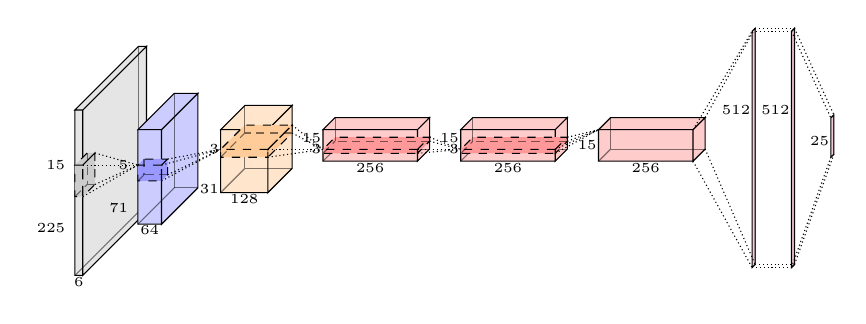
\begin{tikzpicture}
  \tikzset{
    annotated cuboid/.pic={
      \tikzset{%
        every edge quotes/.append style={midway, auto},
        /cuboid/.cd,
        #1
      }
      \draw [\cubeline,every edge/.append style={pic actions, \cubeback, opacity=.5}, pic actions]
      (0,0,0) coordinate (o-\cubelabel) -- ++(-\cubescale*\cubex,0,0) coordinate (a-\cubelabel) -- ++(0,-\cubescale*\cubey,0) coordinate (b-\cubelabel) edge coordinate [pos=1] (g-\cubelabel) ++(0,0,-\cubescale*\cubez)  -- ++(\cubescale*\cubex,0,0) coordinate (c-\cubelabel) -- cycle
      (o-\cubelabel) -- ++(0,0,-\cubescale*\cubez) coordinate (d-\cubelabel) -- ++(0,-\cubescale*\cubey,0) coordinate (e-\cubelabel) edge (g-\cubelabel) -- (c-\cubelabel) -- cycle
      (o-\cubelabel) -- (a-\cubelabel) -- ++(0,0,-\cubescale*\cubez) coordinate (f-\cubelabel) edge (g-\cubelabel) -- (d-\cubelabel) -- cycle;
      ;
    },
    /cuboid/.search also={/tikz},
    /cuboid/.cd,
    width/.store in=\cubex,
    height/.store in=\cubey,
    depth/.store in=\cubez,
    units/.store in=\cubeunits,
    scale/.store in=\cubescale,
    label/.store in=\cubelabel,
    line/.store in=\cubeline,
    backline/.store in=\cubeback,
    width=10,
    height=10,
    depth=10,
    units=cm,
    scale=.1,
    line=draw,
    backline=densely dashed,
    font=\tiny
  }
  
  \pic [fill=gray!20, text=green!50!black, draw=black] at (4,-2) {annotated cuboid={label=A, width=1, height=21, depth=21, units=mm, backline=draw}};

  \node [left,yshift=-1.5cm] at (a-A) {225};
  \node [below,xshift=0.05cm,yshift=0.1cm] at (b-A) {6};

  \pic [fill=gray!40, text=green!50!black, draw=black] at (4,-2.7) {annotated cuboid={label=B, width=1, height=4, depth=4, units=m, line=dashed}};

  \node [left] at (a-B) {15};

  \pic [fill=blue!20, text=green!50!black, draw=black] at (5,-2.25) {annotated cuboid={label=C, width=3, height=12, depth=12, units=mm, backline=draw}};
	
  \node [left,yshift=-1cm] at (a-C) {71};
  \node [below,xshift=0.15cm,yshift=0.1cm] at (b-C) {64};

  \pic [fill=blue!40, text=green!50!black, draw=black] at (5,-2.7) {annotated cuboid={label=D, width=3, height=2, depth=2, units=m, line=dashed}};

  \node [left] at (a-D) {5};

  \pic [fill=orange!20, text=green!50!black, draw=black] at (6.35,-2.25) {annotated cuboid={label=E, width=6, height=8, depth=8, units=m, backline=draw}};

  \node [left,xshift=0.1cm,yshift=-0.75cm] at (a-E) {31};
  \node [below,xshift=0.3cm,yshift=0.1cm] at (b-E) {128};

  \pic [fill=orange!40, text=green!50!black, draw=black] at (6.35,-2.5) {annotated cuboid={label=F, width=6, height=1, depth=8, units=m, line=dashed}};

  \node [left,xshift=0.1cm] at (a-F) {3};

  \pic [fill=red!20, text=green!50!black, draw=black] at (8.25,-2.25) {annotated cuboid={label=G, width=12, height=4, depth=4, units=m, backline=draw}};

  \node [left,xshift=0.1cm,yshift=-0.1cm] at (a-G) {15};
  \node [below,xshift=0.6cm,yshift=0.1cm] at (b-G) {256};

  \pic [fill=red!40, text=green!50!black, draw=black] at (8.25,-2.5) {annotated cuboid={label=H, width=12, height=0.5, depth=4, units=m, line=dashed}};

  \node [left,xshift=0.1cm] at (a-H) {3};

  \pic [fill=red!20, text=green!50!black, draw=black] at (10,-2.25) {annotated cuboid={label=I, width=12, height=4, depth=4, units=m, backline=draw}};

  \node [left,xshift=0.1cm,yshift=-0.1cm] at (a-I) {15};
  \node [below,xshift=0.6cm,yshift=0.1cm] at (b-I) {256};

  \pic [fill=red!40, text=green!50!black, draw=black] at (10,-2.5) {annotated cuboid={label=J, width=12, height=0.5, depth=4, units=m, line=dashed}};

  \node [left,xshift=0.1cm] at (a-J) {3};

  \pic [fill=red!20, text=green!50!black, draw=black] at (11.75,-2.25) {annotated cuboid={label=K, width=12, height=4, depth=4, units=m, backline=draw}};
  
  \node [left,xshift=0.1cm,yshift=-0.2cm] at (a-K) {15};
  \node [below,xshift=0.6cm,yshift=0.1cm] at (b-K) {256};

  
  \pic [fill=purple!20, text=green!50!black, draw=black] at (12.5,-1) {annotated cuboid={label=L, width=0, height=30, depth=1, units=m, backline=draw}};

  \node [left,xshift=0.1cm,yshift=-1cm] at (a-L) {512};

  \pic [fill=purple!20, text=green!50!black, draw=black] at (13,-1) {annotated cuboid={label=M, width=0, height=30, depth=1, units=m, backline=draw}};

  \node [left,xshift=0.1cm,yshift=-1cm] at (a-M) {512};  

  \pic [fill=purple!20, text=green!50!black, draw=black] at (13.5,-2.1) {annotated cuboid={label=N, width=0, height=5, depth=1, units=m, backline=draw}};

  \node [left,xshift=0.1cm,yshift=-0.3cm] at (a-N) {25}; 

  \foreach \point in {c,d,e,o} {
    \draw[densely dotted] (\point-B) -- (a-D);
    \draw[densely dotted] (\point-D) -- (a-F);
    \draw[densely dotted] (\point-F) -- (a-H);
    \draw[densely dotted] (\point-H) -- (a-J);
  	\draw[densely dotted] (\point-J) -- (a-K);
  	\draw[densely dotted] (\point-K) -- (\point-L);
    \draw[densely dotted] (\point-L) -- (\point-M);
    \draw[densely dotted] (\point-M) -- (\point-N);
  }
\end{tikzpicture}
}